\documentclass[a4paper,12pt]{book}
\usepackage[utf8]{inputenc}
\title{}
\author{Rachel Morris}
\date{\today}

\usepackage{rachwidgets}
\usepackage{fancyhdr}
\usepackage{lastpage}
\usepackage{dirtree}
\usepackage{boxedminipage}
\usepackage{colortbl} % cell bg colors

\setcounter{chapter}{4}
\setcounter{section}{0}
\newcommand{\laChapter}{4.1 Definitions, Diagrams, and Inverses\ }
\newcounter{question}

\newcommand{\laClass}{CS 210\ }
\newcommand{\laSemester}{Fall 2017\ }

\pagestyle{fancy}
\fancyhf{}
\lhead{\laClass \laSemester}
\chead{}
\rhead{Ch \laChapter}
\rfoot{\thepage\ of \pageref{LastPage}}
\lfoot{\scriptsize Compiled by Rachel Morris, last updated \today}

\renewcommand{\headrulewidth}{2pt}
\renewcommand{\footrulewidth}{1pt}

\begin{document}

    %\toggletrue{answerkey}
    \togglefalse{answerkey}

    %------------------------------------------------------------------%
    %- Exercise Begin -------------------------------------------------%
    %------------------------------------------------------------------%

    \section{Definitions, Diagrams, and Inverses}

    \subsection{Function Terminology}

    \notonkey{
        \begin{introNOHEAD}{}
            \paragraph{Function:} We use the notation $f : A \to B$ to
                specify a function $f$, which has inputs from the set $A$,
                and outputs from the set $B$. The function associates
                each input in $A$ to one and only one output in $B$.
                \footnote{Discrete Mathematics, Ensley and Crawley}
                The notation $f : A \to B$ can be read as ``$f$ is
                a function from $A$ to $B$".

            \paragraph{Domain:} The Domain is the set of inputs ($A$).

            \paragraph{Codomain:} The Codomain is the set of outputs ($B$).
        \end{introNOHEAD}
    }{}


    % - QUESTION --------------------------------------------------%
    \stepcounter{question}
    \begin{questionNOGRADE}{\thequestion}

        Given the function:

        \begin{center}
            $ g : \mathbb{Z} \to \mathbb{N} $
            \tab ...with the rule... \tab
            $ g(x) = x^{2} $
        \end{center}

        \begin{enumerate}
            \item[a.]   What is the function name?  \solution{ $g$ }{ \vspace{0.5cm} }
            \item[b.]   What is the domain?  \solution{ $\mathbb{Z}$ }{ \vspace{0.5cm} }
            \item[c.]   What is the codomain?  \solution{ $\mathbb{N}$ }{ \vspace{0.5cm} }
            \item[d.]   Is 2 a valid domain value?  \solution{ Yes }{ \vspace{0.5cm} }
            \item[e.]   Is -2 a valid domain value?  \solution{ Yes }{ \vspace{0.5cm} }
            \item[f.]   Is 4 a valid codomain value?  \solution{ Yes }{ \vspace{0.5cm} }
            \item[g.]   Is -4 a valid codomain value?  \solution{ No }{ \vspace{0.5cm} }
        \end{enumerate}

    \end{questionNOGRADE}

    \notonkey{ \newpage }{ \hrulefill }

    \notonkey{
        \begin{introNOHEAD}{}
            To describe a function, you need four items:
            \footnote{Discrete Mathematics, Ensley and Crawley}
            (1) Give the function a name, such as $f$, $g$, and $h$,
            (2) Describe the \textbf{domain},
            (3) Describe the \textbf{codomain},
            (4) Describe the \textbf{rule}.

            \paragraph{Example:}
                Function $f$, with Domain: $\{1, 2, 3\}$ and Codomain: $\{2, 4, 6\}$
                and the Rule:   $f(x) = 2x$.

                \subparagraph{Function diagram:}

                With a diagram, arrows start at an element in the domain,
                and point to an element in the codomain.

                \begin{center}
                    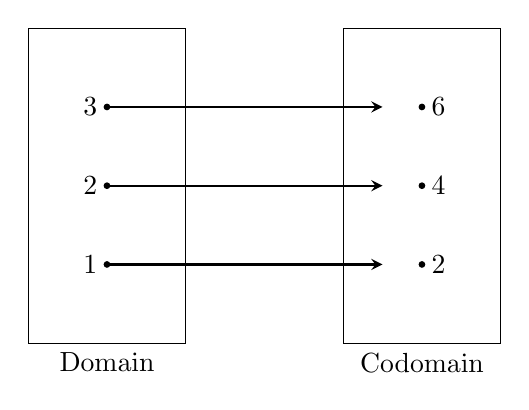
\begin{tikzpicture}[arrow/.style = {thick,-stealth}]
                        \draw[fill=white] (0,0) rectangle (2,4);
                        \draw[fill=white] (4,0) rectangle (6,4);
                        \filldraw (1,1) circle (1pt) node[left] {1};
                        \filldraw (1,2) circle (1pt) node[left] {2};
                        \filldraw (1,3) circle (1pt) node[left] {3};
                        \filldraw (5,1) circle (1pt) node[right] {2};
                        \filldraw (5,2) circle (1pt) node[right] {4};
                        \filldraw (5,3) circle (1pt) node[right] {6};
                        \draw[arrow] (1,1) -- (4.5,1);
                        \draw[arrow] (1,2) -- (4.5,2);
                        \draw[arrow] (1,3) -- (4.5,3);
                        \node [below] at (1,0) {Domain};
                        \node [below] at (5,0) {Codomain};
                    \end{tikzpicture}
                \end{center}
        \end{introNOHEAD}
    }{}

    % - QUESTION --------------------------------------------------%
    \stepcounter{question}
    \begin{questionNOGRADE}{\thequestion}

        \begin{enumerate}
            \item[a.] Define a function where the inputs and outputs are integers,
                and the relationship is that the output is the \textit{square} of the input
                provided to the function.

                \solution{
                    $f : \mathbb{Z} \to \mathbb{Z}$, with $f(x) = x^{2}$
                }{ \vspace{2cm} }

            \item[b.] Draw a diagram of the function. Include 5 values in the
                domain and in the co-domain.
        \end{enumerate}

    \end{questionNOGRADE}

    \notonkey{ \newpage }{ \hrulefill }

    \subsection{Binary Relations}

    \notonkey{
        \begin{introNOHEAD}{}
            A \textbf{binary relation} $R$ consists of three components:
            a domain $A$, a codomain $B$, and a subset of $A \times B$
            called the ``rule" for the relation.
            \footnote{Discrete Mathematics, Ensley and Crawley}

            \paragraph{Example:}
                Domain = $\{1, 2\}$, Codomain = $\{2, 3\}$, \\ and the
                Rule is $\{ (1,2), (1,3), (2,2), (2,3) \}$.

                \begin{center}
                    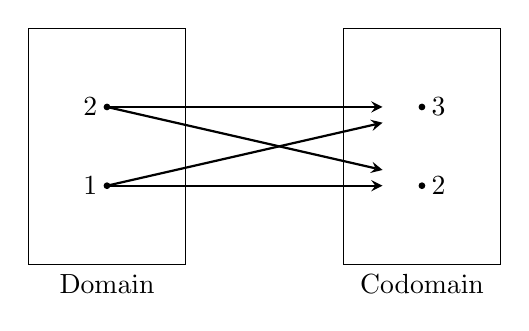
\begin{tikzpicture}[arrow/.style = {thick,-stealth}]
                        \draw[fill=white] (0,0) rectangle (2,3);
                        \draw[fill=white] (4,0) rectangle (6,3);

                        \filldraw (1,1) circle (1pt) node[left] {1};
                        \filldraw (1,2) circle (1pt) node[left] {2};
                        \filldraw (5,1) circle (1pt) node[right] {2};
                        \filldraw (5,2) circle (1pt) node[right] {3};
                        \draw[arrow] (1,1) -- (4.5,1);
                        \draw[arrow] (1,2) -- (4.5,2);
                        \draw[arrow] (1,2) -- (4.5,1.2);
                        \draw[arrow] (1,1) -- (4.5,1.8);
                        \node [below] at (1,0) {Domain};
                        \node [below] at (5,0) {Codomain};
                    \end{tikzpicture}
                \end{center}
        \end{introNOHEAD}
    }{}

    % - QUESTION --------------------------------------------------%
    \stepcounter{question}
    \begin{questionNOGRADE}{\thequestion}

        Finish the arrow diagram for the following Binary Relation.

        Domain: $\{ 1, 2, 3, 4, 5 \}$

        Codomain: $\{ 1, 2, 3, 4, 5 \}$

        Rule: \{ (1,5), (2,3), (3,3), (4,2), (5,1) \}

        \begin{center}
            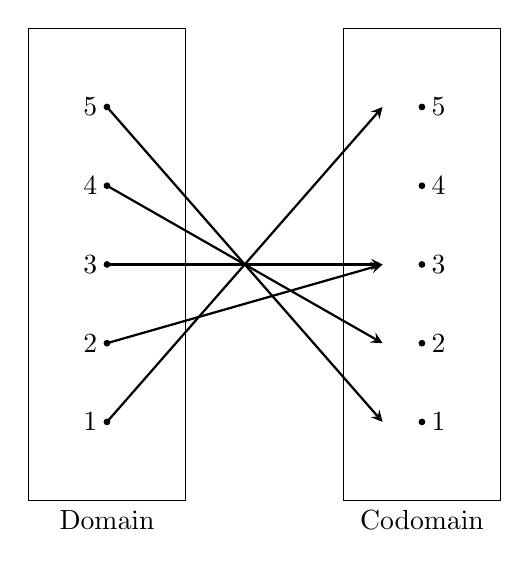
\begin{tikzpicture}[arrow/.style = {thick,-stealth}]
                \draw (0,0) rectangle (2,6);
                \draw (4,0) rectangle (6,6);

                \filldraw (1,1) circle (1pt) node[left] {1};
                \filldraw (1,2) circle (1pt) node[left] {2};
                \filldraw (1,3) circle (1pt) node[left] {3};
                \filldraw (1,4) circle (1pt) node[left] {4};
                \filldraw (1,5) circle (1pt) node[left] {5};

                \filldraw (5,1) circle (1pt) node[right] {1};
                \filldraw (5,2) circle (1pt) node[right] {2};
                \filldraw (5,3) circle (1pt) node[right] {3};
                \filldraw (5,4) circle (1pt) node[right] {4};
                \filldraw (5,5) circle (1pt) node[right] {5};
                
                \solution{ \draw[arrow] (1,1) -- (4.5,5); }{}
                \solution{ \draw[arrow] (1,5) -- (4.5,1); }{}
                \solution{ \draw[arrow] (1,2) -- (4.5,3); }{}
                \solution{ \draw[arrow] (1,4) -- (4.5,2); }{}
                \solution{ \draw[arrow] (1,3) -- (4.5,3); }{}
                
                \node [below] at (1,0) {Domain};
                \node [below] at (5,0) {Codomain};
            \end{tikzpicture}
        \end{center}

    \end{questionNOGRADE}

    \notonkey{ \newpage }{ \hrulefill }

    % - QUESTION --------------------------------------------------%
    \stepcounter{question}
    \begin{questionNOGRADE}{\thequestion}

        Finish the arrow diagram for the following Binary Relation.

        ~\\
        Domain: $\wp( \{1, 2, 3\} )$, the Power Set of \{1, 2, 3\}.

        ~\\
        Codomain: The set $B$ = \{0, 1, 2, 3, 4, 5, 6, 7\}.

        ~\\
        Rule: $(S,n) \in \mathbb{R}$ \\
        This means that $n$ is the \textbf{sum} of elements in the the set
        $S$ given as an input. For example, with the input set \{1, 2\},
        the output will be $1 + 2$, or 3.

        \begin{center}
            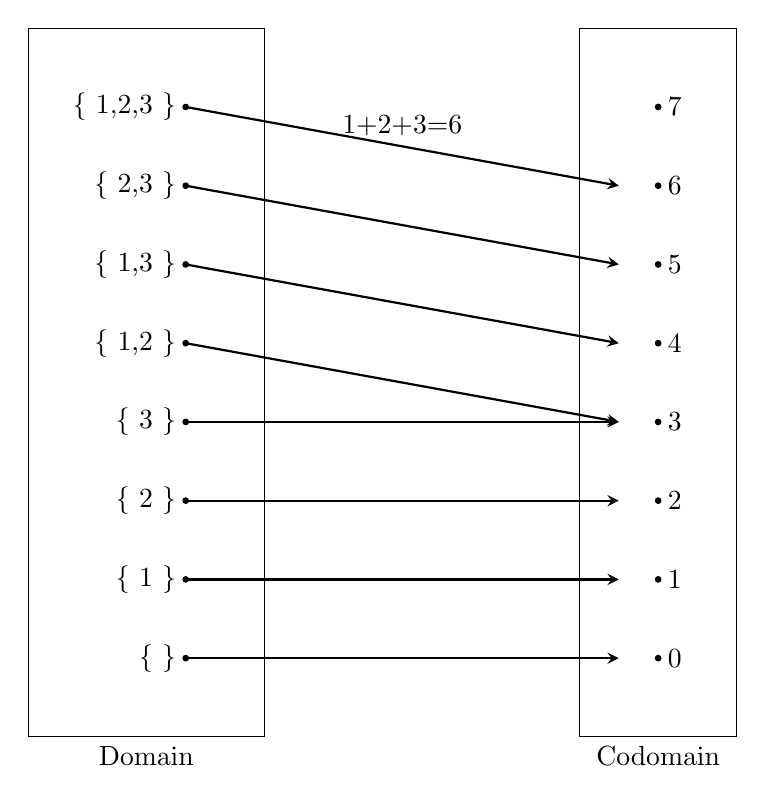
\begin{tikzpicture}[arrow/.style = {thick,-stealth}]
                \draw (0,0) rectangle (3,9);
                \draw (7,0) rectangle (9,9);

                \filldraw (2,1) circle (1pt) node[left] { \{ \} };
                \filldraw (2,2) circle (1pt) node[left] { \{ 1 \} };
                \filldraw (2,3) circle (1pt) node[left] { \{ 2 \} };
                \filldraw (2,4) circle (1pt) node[left] { \{ 3 \} };
                \filldraw (2,5) circle (1pt) node[left] { \{ 1,2 \} };
                \filldraw (2,6) circle (1pt) node[left] { \{ 1,3 \} };
                \filldraw (2,7) circle (1pt) node[left] { \{ 2,3 \} };
                \filldraw (2,8) circle (1pt) node[left] { \{ 1,2,3 \} };

                \filldraw (8,1) circle (1pt) node[right] {0};
                \filldraw (8,2) circle (1pt) node[right] {1};
                \filldraw (8,3) circle (1pt) node[right] {2};
                \filldraw (8,4) circle (1pt) node[right] {3};
                \filldraw (8,5) circle (1pt) node[right] {4};
                \filldraw (8,6) circle (1pt) node[right] {5};
                \filldraw (8,7) circle (1pt) node[right] {6};
                \filldraw (8,8) circle (1pt) node[right] {7};

                \draw[arrow] (2,8) -- (7.5,7) node[pos=0.5,above] {1+2+3=6};
                \solution{ \draw[arrow] (2,1) -- (7.5,1); }{}
                \solution{ \draw[arrow] (2,2) -- (7.5,2); }{}
                \solution{ \draw[arrow] (2,3) -- (7.5,3); }{}
                \solution{ \draw[arrow] (2,4) -- (7.5,4); }{}
                \solution{ \draw[arrow] (2,5) -- (7.5,4); }{}
                \solution{ \draw[arrow] (2,6) -- (7.5,5); }{}
                \solution{ \draw[arrow] (2,7) -- (7.5,6); }{}

                \node [below] at (1.5,0) {Domain};
                \node [below] at (8,0) {Codomain};
            \end{tikzpicture}
        \end{center}

    \end{questionNOGRADE}

    \notonkey{ \newpage }{ \hrulefill }

    \notonkey{
        \begin{introNOHEAD}{}
            A function $f : A \to B$ is a binary relation with domain $A$
            and codomain $B$ with the property that for every $x \in A$,
            there is \textbf{exactly one} element $y \in B$ for which
            $(x, y) \in  f$.
            \footnote{Discrete Mathematics, Ensley and Crawley}

            ~\\
            Bluntly, the pair $(x,y)$ denotes that a line begins at
            element $x$ from the domain, and points to the element
            $y$ in the codomain.
        \end{introNOHEAD}
    }{}

    % - QUESTION --------------------------------------------------%
    \stepcounter{question}
    \begin{questionNOGRADE}{\thequestion}

        Identify which of the following relations are also functions.
        Explain why not, if the relation is not a function. Also complete
        the diagrams given.
        % 4.1 Example 11 %

        \begin{enumerate}
            \item[a.]   Relation $R_{1}$
                \footnotesize
                \\ \tab Domain:     The set $\mathbb{S}$ of all students at your college this semester.
                \\ \tab Codomain:   The set $\mathbb{C}$ of all classes offered at your college this semester.
                \\ \tab Rule:       $(x,y)$ is in $R_{1}$ if student $x$ is enrolled in class $y$ this semester.
                \normalsize

                Let's use a small sample set. Fill it out to help you figure out
                if this is a function. \solution{ Not a function; a student can take more than 1 class. }{}

                \begin{center}
                    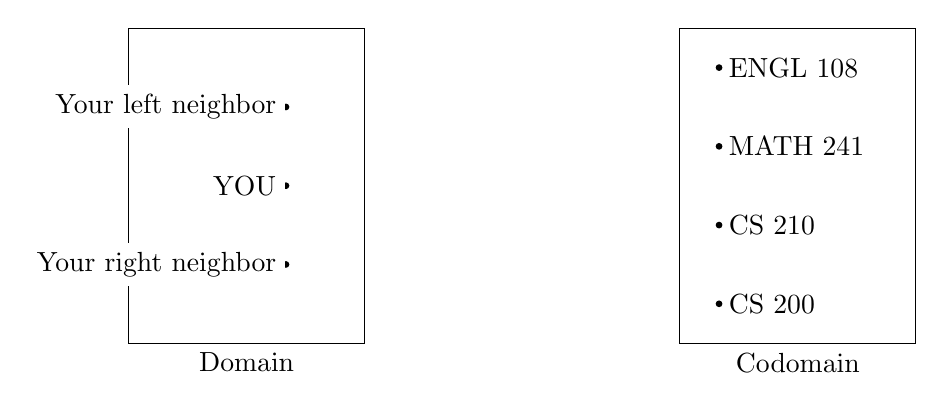
\begin{tikzpicture}[arrow/.style = {thick,-stealth}]
                        \draw (0,0) rectangle (3,4);
                        \draw (7,0) rectangle (10,4);

                        \filldraw (2,1) circle (1pt) node[left,fill=white] { Your right neighbor };
                        \filldraw (2,2) circle (1pt) node[left,fill=white] { YOU };
                        \filldraw (2,3) circle (1pt) node[left,fill=white] { Your left neighbor };

                        \filldraw (7.5,0.5) circle (1pt) node[right] {CS 200};
                        \filldraw (7.5,1.5) circle (1pt) node[right] {CS 210};
                        \filldraw (7.5,2.5) circle (1pt) node[right] {MATH 241};
                        \filldraw (7.5,3.5) circle (1pt) node[right] {ENGL 108};

                        %\draw[arrow] (2,8) -- (7.5,7) node[pos=0.5,above] {1+2+3=6};
                        %\solution{ \draw[arrow] (2,1) -- (7.5,1); }{}

                        \node [below] at (1.5,0) {Domain};
                        \node [below] at (8.5,0) {Codomain};
                    \end{tikzpicture}
                \end{center}

            \item[b.]   Relation $R_{2}$
                \footnotesize
                \\ \tab Domain:  The set $A$ = \{1, 2, 3\}.
                \tab Codomain:   The set $B$ = \{2, 4, 6\}.
                \tab Rule:       $(x,y)$ is in $R_{2}$ if $2x = y$.
                \normalsize
                \solution{ This is a function }{}

                \begin{center}
                    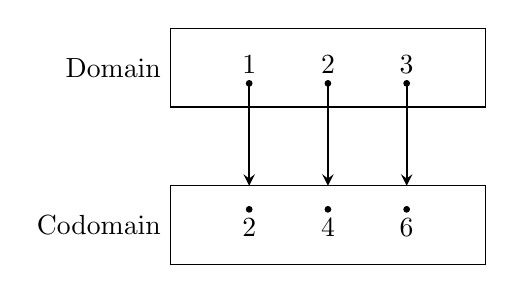
\begin{tikzpicture}[arrow/.style = {thick,-stealth}]
                        \draw (0,0) rectangle (4,1);
                        \draw (0,-1) rectangle (4,-2);

                        \filldraw (1, 0.3) circle (1pt) node[above] {1};
                        \filldraw (2, 0.3) circle (1pt) node[above] {2};
                        \filldraw (3, 0.3) circle (1pt) node[above] {3};

                        \filldraw (1, -1.3) circle (1pt) node[below] {2};
                        \filldraw (2, -1.3) circle (1pt) node[below] {4};
                        \filldraw (3, -1.3) circle (1pt) node[below] {6};

                        \solution{ \draw[arrow] (1, 0.3) -- (1, -1.0); }{}
                        \solution{ \draw[arrow] (2, 0.3) -- (2, -1.0); }{}
                        \solution{ \draw[arrow] (3, 0.3) -- (3, -1.0); }{}

                        \node [left] at (0,0.5) {Domain};
                        \node [left] at (0,-1.5) {Codomain};
                    \end{tikzpicture}
                \end{center}

        \end{enumerate}

    \end{questionNOGRADE}

    \notonkey{ \newpage }{ \hrulefill }

    % - QUESTION --------------------------------------------------%
    \stepcounter{question}
    \begin{questionNOGRADE}{\thequestion}

        Identify which of the following relations are also functions.
        Explain why not, if the relation is not a function. Also complete
        the diagrams given.

        \begin{enumerate}
            \item[a.]   Relation $R_{3}$
                \footnotesize
                \\ \tab Domain:  The set $A$ = \{1, 2, 3\}.
                \tab Codomain:   The set $B$ = \{2, 4, 6\}.
                \tab Rule:       \{ (1,6), (2,2), (3,4) \}
                \normalsize

                Let's use a small sample set. Fill it out to help you figure out
                if this is a function.
                \solution{ This is a function. }{}

                \begin{center}
                    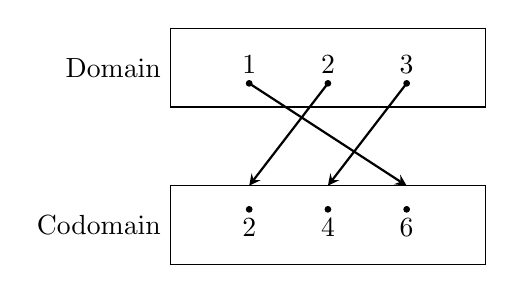
\begin{tikzpicture}[arrow/.style = {thick,-stealth}]
                        \draw (0,0) rectangle (4,1);
                        \draw (0,-1) rectangle (4,-2);

                        \filldraw (1, 0.3) circle (1pt) node[above] {1};
                        \filldraw (2, 0.3) circle (1pt) node[above] {2};
                        \filldraw (3, 0.3) circle (1pt) node[above] {3};

                        \filldraw (1, -1.3) circle (1pt) node[below] {2};
                        \filldraw (2, -1.3) circle (1pt) node[below] {4};
                        \filldraw (3, -1.3) circle (1pt) node[below] {6};

                        \solution{ \draw[arrow] (1, 0.3) -- (3, -1.0); }{}
                        \solution{ \draw[arrow] (2, 0.3) -- (1, -1.0); }{}
                        \solution{ \draw[arrow] (3, 0.3) -- (2, -1.0); }{}

                        \node [left] at (0,0.5) {Domain};
                        \node [left] at (0,-1.5) {Codomain};
                    \end{tikzpicture}
                \end{center}

            \item[b.]   Relation $R_{4}$
                \footnotesize
                \\ \tab Domain:     The set $A$ = \{1, 2, 3, 4, 5, 6\}.
                \tab Codomain:   The same set $A$.
                \tab Rule:       $(x,y)$ is in $R_{3}$ if $x-1 = y$.
                \normalsize
                \solution{ This is not a function; 1 doesn't point to anything, and 6 isn't pointed to by anything. }{}

                \begin{center}
                    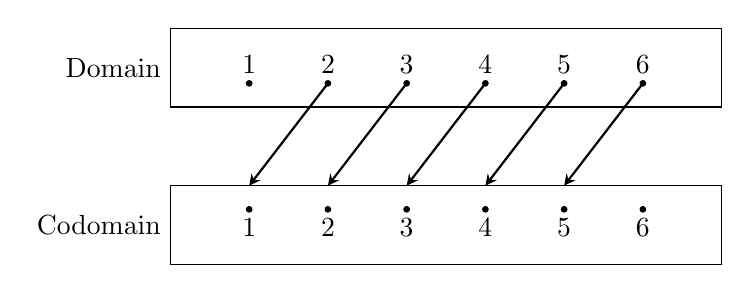
\begin{tikzpicture}[arrow/.style = {thick,-stealth}]
                        \draw (0,0) rectangle (7,1);
                        \draw (0,-1) rectangle (7,-2);

                        \filldraw (1, 0.3) circle (1pt) node[above] {1};
                        \filldraw (2, 0.3) circle (1pt) node[above] {2};
                        \filldraw (3, 0.3) circle (1pt) node[above] {3};
                        \filldraw (4, 0.3) circle (1pt) node[above] {4};
                        \filldraw (5, 0.3) circle (1pt) node[above] {5};
                        \filldraw (6, 0.3) circle (1pt) node[above] {6};

                        \filldraw (1, -1.3) circle (1pt) node[below] {1};
                        \filldraw (2, -1.3) circle (1pt) node[below] {2};
                        \filldraw (3, -1.3) circle (1pt) node[below] {3};
                        \filldraw (4, -1.3) circle (1pt) node[below] {4};
                        \filldraw (5, -1.3) circle (1pt) node[below] {5};
                        \filldraw (6, -1.3) circle (1pt) node[below] {6};

                        \solution{ \draw[arrow] (2, 0.3) -- (1, -1.0); }{}
                        \solution{ \draw[arrow] (3, 0.3) -- (2, -1.0); }{}
                        \solution{ \draw[arrow] (4, 0.3) -- (3, -1.0); }{}
                        \solution{ \draw[arrow] (5, 0.3) -- (4, -1.0); }{}
                        \solution{ \draw[arrow] (6, 0.3) -- (5, -1.0); }{}

                        \node [left] at (0,0.5) {Domain};
                        \node [left] at (0,-1.5) {Codomain};
                    \end{tikzpicture}
                \end{center}

        \end{enumerate}

    \end{questionNOGRADE}

    \notonkey{ \newpage }{ \hrulefill }

    \subsection{Inverse Relations}

    \notonkey{
        \begin{introNOHEAD}{}
            Given a relation $R$ with domain $A$ and codomain $B$,
            the relation $R_{-1}$ (read ``$R$ inverse") with domain $B$
            and codomain $A$ is called the \textbf{inverse} of $R$,
            and is defined so that
            \begin{center}
                $(x,y) \in R$ \tab if and only if \tab $(y,x) \in R^{-1}$
            \end{center}

            Also note that the inverse of $R^{-1}$ is $R$.
            \footnote{Discrete Mathematics, Ensley and Crawley}
        \end{introNOHEAD}
    }{}

    % - QUESTION --------------------------------------------------%
    \stepcounter{question}
    \begin{questionNOGRADE}{\thequestion}

        Draw the inverse of each diagram.
        Identify if the original, and/or the inverse, are functions.

        \begin{enumerate}
            \item[a.] ~\\
                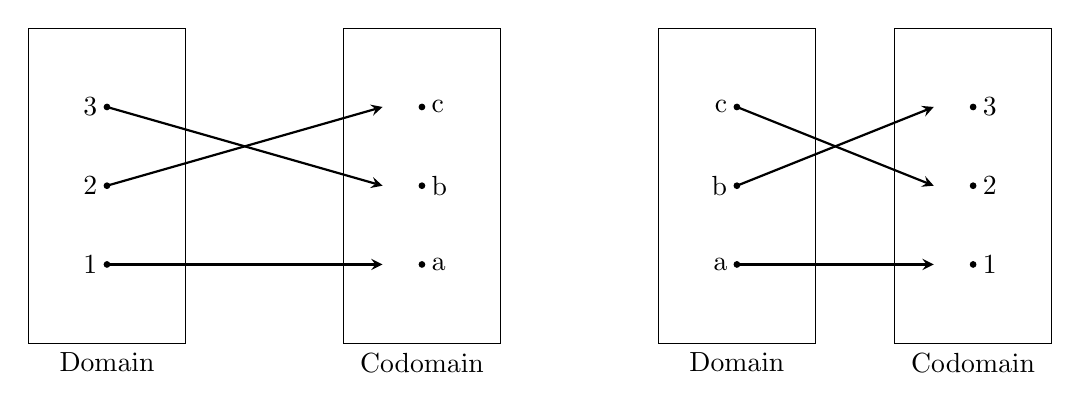
\begin{tikzpicture}[arrow/.style = {thick,-stealth}]
                    \draw (0,0) rectangle (2,4);
                    \draw (4,0) rectangle (6,4);

                    \filldraw (1, 1) circle (1pt) node[left] {1};
                    \filldraw (1, 2) circle (1pt) node[left] {2};
                    \filldraw (1, 3) circle (1pt) node[left] {3};

                    \filldraw (5, 1) circle (1pt) node[right] {a};
                    \filldraw (5, 2) circle (1pt) node[right] {b};
                    \filldraw (5, 3) circle (1pt) node[right] {c};

                    \draw[arrow] (1, 1) -- (4.5, 1);
                    \draw[arrow] (1, 2) -- (4.5, 3);
                    \draw[arrow] (1, 3) -- (4.5, 2);

                    \node [below] at (1,0) {Domain};
                    \node [below] at (5,0) {Codomain};

                    \solution{
                        \draw (8,0) rectangle (10,4);
                        \draw (11,0) rectangle (13,4);

                        \filldraw (9, 1) circle (1pt) node[left] {a};
                        \filldraw (9, 2) circle (1pt) node[left] {b};
                        \filldraw (9, 3) circle (1pt) node[left] {c};

                        \filldraw (12, 1) circle (1pt) node[right] {1};
                        \filldraw (12, 2) circle (1pt) node[right] {2};
                        \filldraw (12, 3) circle (1pt) node[right] {3};

                        \solution{ \draw[arrow] (9, 1) -- (11.5, 1); }{}
                        \solution{ \draw[arrow] (9, 2) -- (11.5, 3); }{}
                        \solution{ \draw[arrow] (9, 3) -- (11.5, 2); }{}

                        \node [below] at (9,0) {Domain};
                        \node [below] at (12,0) {Codomain};
                    }{}
                \end{tikzpicture}
                \solution{ Both are functions. }{}
                ~\\~\\

            \item[b.] ~\\
                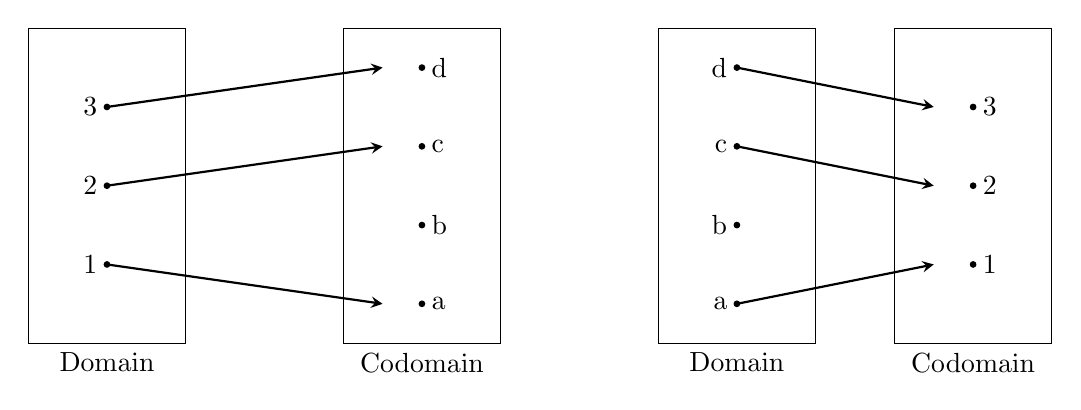
\begin{tikzpicture}[arrow/.style = {thick,-stealth}]
                    \draw (0,0) rectangle (2,4);
                    \draw (4,0) rectangle (6,4);

                    \draw[arrow] (1, 1) -- (4.5, 0.5);
                    \draw[arrow] (1, 2) -- (4.5, 2.5);
                    \draw[arrow] (1, 3) -- (4.5, 3.5);

                    \filldraw (1, 1) circle (1pt) node[left] {1};
                    \filldraw (1, 2) circle (1pt) node[left] {2};
                    \filldraw (1, 3) circle (1pt) node[left] {3};

                    \filldraw (5, 0.5) circle (1pt) node[right] {a};
                    \filldraw (5, 1.5) circle (1pt) node[right] {b};
                    \filldraw (5, 2.5) circle (1pt) node[right] {c};
                    \filldraw (5, 3.5) circle (1pt) node[right] {d};
                    
                    \node [below] at (1,0) {Domain};
                    \node [below] at (5,0) {Codomain};

                    

                    \solution{
                        \draw (8,0) rectangle (10,4);
                        \draw (11,0) rectangle (13,4);

                        \solution{ \draw[arrow] (9, 0.5) -- (11.5, 1); }{}
                        \solution{ \draw[arrow] (9, 2.5) -- (11.5, 2); }{}
                        \solution{ \draw[arrow] (9, 3.5) -- (11.5, 3); }{}

                        \filldraw (12, 1) circle (1pt) node[right] {1};
                        \filldraw (12, 2) circle (1pt) node[right] {2};
                        \filldraw (12, 3) circle (1pt) node[right] {3};

                        \filldraw (9, 0.5) circle (1pt) node[left] {a};
                        \filldraw (9, 1.5) circle (1pt) node[left] {b};
                        \filldraw (9, 2.5) circle (1pt) node[left] {c};
                        \filldraw (9, 3.5) circle (1pt) node[left] {d};
                        
                        \node [below] at (9,0) {Domain};
                        \node [below] at (12,0) {Codomain};
                    }{}
                \end{tikzpicture}
                \solution{ The original is a function, but the inverse is not a function. }{}
        \end{enumerate}
        
    \end{questionNOGRADE}




\end{document}








